\documentclass[11pt]{article}

\usepackage[spanish,activeacute]{babel}
\usepackage{amsfonts}
\usepackage{graphicx}
\usepackage{whilecode2}


    \title{\textbf{Practica 4}}
    \author{Carmen Alonso Jimenez}
    \date{\today}
    
    \addtolength{\topmargin}{-4cm}
    \addtolength{\textheight}{4cm}
    %\usepackage[spanish]{babel}
    \usepackage[a4paper, margin=3cm, top=5mm, bottom=15mm]{geometry}
    \usepackage{graphicx}
    \usepackage{tikz}

\begin{document}

\maketitle
\thispagestyle{plain}
\setlength{\parskip}{6pt}

\section{Create the simplest WHILE program that computes the diverge function (with
zero arguments) and compute the codification of its code}
	Q = (0,s)
   \\ s:
	
\begin{whilecode}[H]

$X_2 \Assig X_1 + 1$\;
 \While{$X_2 \not = 0$}{

 \DefaultVar{1}\Assig 0

 }
\end{whilecode}
\begin{figure}[htp]
\centering
\includegraphics[scale=0.70]{talfuma/ejercicio1_practica4.png}
\caption{}
\label{}
\end{figure}
\section{Create an Octave script that enumerates all the vectors.}
\begin{verbatim}
   function printNvectors(N)
	for i=0:N-1
	disp([’(’ num2str(godeldecoding(i))’)’])
	end
end
    \end{verbatim}
    
\begin{figure}[htp]
\centering
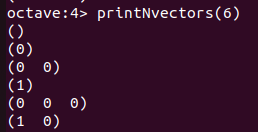
\includegraphics[scale=1.00]{talfuma/Ejercicio2_practica4.png}
\caption{}
\label{}
\end{figure}
\section{Create an Octave script that enumerates all the WHILE programs.}
 \begin{verbatim}
    function printNwhilePrograms(N)

    for i=1:inf
        N2WHILE(i)
    end
    
    end
    \end{verbatim}
    
 \begin{figure}[htp]
\centering
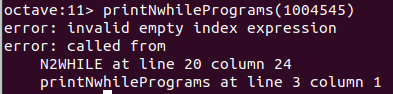
\includegraphics[scale=1.00]{talfuma/ejercicio3_Practica4.png}
\caption{}
\label{}
\end{figure}   

\end{document}